% !TEX root = ../YourName-Dissertation.tex

\chapter{A Few \LaTeX\ Tips} \label{chapter1:introduction}

\section{This is a Section}
After discussing the overall structure, let's throw in a table.

\subsection{A Table}
Units are essential to any quantifiable measure. Newton's second law in scalar form, $F = ma$, provides for the formulation of a consistent and unambiguous system of units.  We will use both \acro{U.S.} Customary units and \acro{SI} units (International System\footnote{\acro{SI} has been adopted as the abbreviation for the French \emph{Le Syst\`{e}me International d'Unit\'{e}s}.}) as shown in Table~\ref{Ch1-table: US Customary and SI Unit Systems}. This is a url \url{https://psu.instructure.com/courses/1929919}.
%%%%
\begin{table}[ht]
\caption{\label{Ch1-table: US Customary and SI Unit Systems}\acro{U.S.} Customary and \acro{SI} unit systems.}
\begin{minipage}{\textwidth}
\centering
\renewcommand{\footnoterule}{\vspace{-7pt}\rule{0pt}{0pt}}
\renewcommand{\arraystretch}{1.2}
\begin{tabular}{l l l}
\toprule
& \multicolumn{2}{c}{\textbf{System of units}}\\
\cmidrule{2-3}
\multicolumn{1}{l}{\textbf{Base dimension}} & \emph{\acro{U.S.} Customary} & \emph{\acro{SI}} \\ \midrule
%%
\qquad force & pound $(\text{lb})$ & newton\footnote{derived unit} $(\text{N})
\equiv \np[kg\text{-}m/\text{s}^{\text{2}}]{\mbox{}}$ \\
%%
%\panel{l}{mass} & \panel{l}{$\text{slug}^{\textit{a}} \equiv \text{lb}\cdot\text{s}^2/\text{ft}$} & \panel{l}{kilogram (kg)} \\
\qquad mass & $\text{slug}^{\textit{a}} \equiv \np[lb\text{-}s^2/ft]{\mbox{}}$ & kilogram $(\text{kg})$ \\
%%
\qquad length & foot $(\text{ft})$ & meter $(\text{m})$ \\
%%
\qquad time & second $(\text{s})$ & second $(\text{s})$ \\ \bottomrule
\end{tabular}
\end{minipage}
\end{table}
%%%%


\subsection{This is a Subsection}

We hold these truths to be self-evident, that all men are created equal,  that they are endowed by their Creator with certain unalienable Rights,  that among these are Life, Liberty and the pursuit of Happiness. --That to secure these  rights, Governments are instituted among Men, deriving their just powers  from the consent of the governed, --That whenever any Form of Government  becomes destructive of these ends, it is the Right of the People to alter  or to abolish it, and to institute new Government, laying its foundation on  such principles and organizing its powers in such form, as to them shall  seem most likely to effect their Safety and Happiness. Prudence, indeed, will dictate that Governments long established should not  be changed for light and transient causes; and accordingly all experience  hath shewn, that mankind are more disposed to suffer, while evils are  sufferable, than to right themselves by abolishing the forms to which they  are accustomed.\cite{BhattacharyaJames-1999-A-Theory-of-Thi-0,RimrottJanabi-Sharifi-1992-A-Torque-Free-F-0,DaviesMoon-1993-3-D-Spatial-Cha-0,Tonkin-1980-A-Basic-Attitud-0,Matsumoto-1984-A-Chaotic-Attra-0,MacKay-1988-A-Criterion-for-0,FreundNix-1996-A-Critical-Thic-0,MarsdenHolmes-1979-A-Horseshoe-in--0,Koiller-1984-A-Mechanical-Sy-0,TsiotrasLonguski-1995-A-New-Parameter-0,ShimadaNagashima-1979-A-Numerical-App-0,HsuLee-1971-A-Stability-Stu-0,Muller-PfeifferKranenburg-1992-A-Two-Dimension-0,HashinShtrikman-1963-A-Variational-A-0,Junkins-1997-Adventures-on-t-0}
%%%
\begin{figure}%[htb]
    \centering
    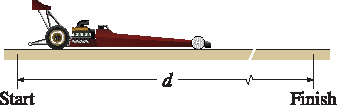
\includegraphics[scale=1.5]{Chapter-1/Figures/dragster}
    \caption{This is a figure with a caption in a floating \texttt{figure} environment.}
    \label{Ch1-figure: dragster}
\end{figure}
%%%


\subsection{Some Equations}
The \acro{FBD} of the box as it tips over the corner is shown at the bottom right, where we have chosen to use polar coordinates for writing the Newton-Euler equations. The Newton-Euler equations corresponding to this \acro{FBD} are
%%
\begin{alignat}{2}
\label{eq: Sum Fx}
&\sum F_{r}\!: \quad & N - mg \cos\theta &= m a_{Gr}, \\
\label{eq: Sum Fy}
&\sum F_{\theta}\!: \quad & mg \sin\theta - F &= m a_{G\theta}, \\
\label{eq: Sum MG}
&\sum M_{G}\!: \quad & F \frac{h}{2} &= I_{G} \alpha,
\end{alignat}
%%
where $I_G = \frac{1}{12}m \left( h^2 + h^2 \right) = \frac{1}{6} m h^2$. Now writing the acceleration of $G$ in polar coordinates, we have
\[
\bv{a}_G = \left( \ddot{r} - r \dot{\theta}^2 \right) \uv{r} + \left( r \ddot{\theta} + 2 \dot{r} \dot{\theta} \right) \uv{\theta} = - \frac{h}{2} \dot{\theta}^2 \,\uv{r} + \frac{h}{2} \ddot{\theta} \,\uv{\theta},
\]
where we have used the fact that the distance from $A$ to $G$ is $r = h/2$ and the fact that $r$ is a constant. Substituting the acceleration components into Eqs.~\eqref{eq: Sum Fx} and~\eqref{eq: Sum Fy}, we obtain
%%
\begin{align}
\label{eq: Sum Fx w/ KE}
N - mg \cos\theta &= -m \frac{h}{2} \dot{\theta}^2, \\
\label{eq: Sum Fy w/ KE}
mg \sin\theta - F &= m \frac{h}{2} \ddot{\theta}.
\end{align}
%%
Solving Eq.~\eqref{eq: Sum Fy w/ KE} for $F$ and substituting it into Eq.~\eqref{eq: Sum MG} and the solving for $\ddot{\theta}$, we obtain
%%
\begin{equation}
\label{eq: angular accel}
\frac{h}{2} \left( mg \sin\theta - m \frac{h}{2} \ddot{\theta} \right) = \frac{1}{6} m h^2 \ddot{\theta}
\quad \Rightarrow \quad
\ddot{\theta} = \frac{6g}{5h} \sin\theta.
\end{equation}
%%
This expression can be substituted into Eq.~\eqref{eq: Sum Fy w/ KE} to obtain $F$ as a function of $\theta$ as
%%
\begin{equation}
\label{eq: F(theta)}
F = mg \sin\theta - m \frac{h}{2} \left( \frac{6g}{5h} \sin\theta \right) = \frac{2}{5} mg \sin\theta.
\end{equation}
%%
Equation~\eqref{eq: Sum Fx w/ KE} tells us that to find $N$ as a function of $\theta$, we need to find $\dot{\theta}$ as a function of $\theta$. This can be done either by applying the work-energy principle or by integrating the expression for $\ddot{\theta}$ in Eq.~\eqref{eq: angular accel}---we will do the latter.

Invoking the chain rule in Eq.~\eqref{eq: angular accel} and integrating, we obtain
%%
\begin{multline}
\label{eq: integrate ang accel}
\ddot{\theta} = \dot{\theta} \frac{d\dot{\theta}}{d\theta} = \frac{6g}{5h} \sin\theta
\quad \Rightarrow \quad
\int_0^{\dot{\theta}} \dot{\theta} \, d\dot{\theta} = \frac{6g}{5h} \int_0^\theta \sin\theta \,d\theta \\
\Rightarrow \quad
\frac{\dot{\theta}^2}{2} = -\frac{6g}{5h} \cos\theta \biggr|_0^\theta = \frac{6g}{5h} \left( 1 - \cos\theta \right)
\quad \Rightarrow \quad
\dot{\theta}^2 = \frac{12g}{5h} \left( 1 - \cos\theta \right).
\end{multline}
%%
Substituting the expression for $\dot{\theta}^2$ in  Eq.~\eqref{eq: integrate ang accel} into Eq.~\eqref{eq: Sum Fx w/ KE} and then solving for $N$, we obtain
%%
\begin{equation}
\label{eq: N(theta)}
N = mg \cos\theta - m \frac{h}{2} \left[ \frac{12g}{5h} \left( 1 - \cos\theta \right) \right] = \frac{1}{5} mg \left( 11 \cos\theta - 6 \right).
\end{equation}
%%

Now, the box will start to slip on the corner when $F = \mu_s N$. Using the expressions for $F$ and $N$ as functions of $\theta$ in Eqs.~\eqref{eq: F(theta)} and~\eqref{eq: N(theta)} in this force law, we obtain
%%
\begin{multline}
\label{eq: theta eqn}
\frac{2}{5} mg \sin\theta = \frac{\mu_s}{5} m g \left( 11\cos\theta - 6 \right)
\quad \Rightarrow \quad
2\sin\theta = \mu_s \left( 11\cos\theta - 6 \right) \\
\Rightarrow \quad \frac{2}{\mu_s} \sin\theta = 11 \cos\theta - 6
\quad \Rightarrow \quad
\frac{2}{\mu_s} \sin\theta = 11 \cos\theta - 6 \\
\Rightarrow \quad \frac{2}{11} \left( \frac{1}{\mu_s} \sin\theta + 3 \right) = \cos\theta.
\end{multline}
%%
To solve the last of Eq.~\eqref{eq: theta eqn}, we let $\cos\theta = \sqrt{1 - \sin^2\theta}$, square both sides, and then rearrange to obtain a quadratic equation in $\sin\theta$ as follows
%%
\begin{multline}
\frac{4}{121} \left( \frac{1}{\mu_s} \sin\theta + 3 \right)^{\!2} = 1 - \sin^2\theta
\quad \Rightarrow \quad
\frac{4}{121} \left( \frac{1}{\mu_s^2} \sin^2\theta + \frac{6}{\mu_s} \sin\theta + 9 \right) = 1 - \sin^2\theta \\
\Rightarrow \quad
\left( \frac{4}{121\mu_s^2} + 1 \right) \sin^2\theta + \frac{24}{121\mu_s} \sin\theta - \left( \frac{36}{121} - 1 \right) = 0 \\
\Rightarrow \quad
\left( 4 + 121\mu_s^2 \right) \sin^2\theta + 24 \mu_s \sin\theta - 85 \mu_s^2 = 0.
\end{multline}
%%
Applying the quadratic formula, we obtain
%%
\begin{align*}
\sin\theta &=
\frac{
-24\mu_s \pm \sqrt{ (24\mu_s)^2 - 4 \left(4 + 121\mu_s^2\right)\left(-85\mu_s^2\right) }
}
{
2 \left( 4 + 121\mu_s^2 \right)
} \\
&=
\frac{
-24\mu_s \pm \sqrt{ 484\mu_s^2 \left(4 + 85\mu_s^2\right) }
}
{
2 \left( 4 + 121\mu_s^2 \right)
} \\
&=
\frac{
-24\mu_s \pm 22\mu_s \sqrt{ 4 + 85\mu_s^2 }
}
{
2 \left( 4 + 121\mu_s^2 \right)
} \\
&=
\frac{
\mu_s \left( -12 \pm 11 \sqrt{ 4 + 85\mu_s^2 } \right)
}
{
4 + 121\mu_s^2
}.
\end{align*}
%%
Therefore, the angle at which the box slips is
\[
\theta = \sin^{-1} \left[ \frac{
\mu_s \left( -12 \pm 11 \sqrt{ 4 + 85\mu_s^2 } \right)
}
{
4 + 121\mu_s^2
} \right].
\]
For example, for $\mu_s = 1/3$, the two angles are $\theta = 32.78^\circ$ for the plus root and $\theta = -90^\circ$ for the minus root. Obviously, the physically meaningful result is the angle corresponding to the plus root.


\subsubsection{This is a Subsubsection}
\label{Ch1 subsection on SMAs}

We hold these truths subsubsection~\ref{Ch1 subsection on SMAs} to be self-evident, that all men are created equal,  that they are endowed by their Creator with certain unalienable Rights,  that among these are Life, Liberty and the pursuit of Happiness. That to secure these  rights, Governments are instituted among Men, deriving their just powers  from the consent of the governed, That whenever any Form of Government  becomes destructive of these ends, it is the Right of the People to alter  or to abolish it, and to institute new Government, laying its foundation on  such principles and organizing its powers in such form, as to them shall  seem most likely to effect their Safety and Happiness. Prudence, indeed, will dictate that Governments long established should not  be changed for light and transient causes; and accordingly all experience  hath shewn, that mankind are more disposed to suffer, while evils are  sufferable, than to right themselves by abolishing the forms to which they  are accustomed~\cite{SmithDavenport-1988-A-Perturbation--0,Ketema-1992-A-Physical-Inte-0,GraesserCozzarelli-1994-A-Proposed-Thre-0,RichardsonMitchell-1999-A-Simplified-Va-0,MitchellRichardson-1999-A-Simplified-Va-0,Parks-1967-A-Stability-Cri-0}.
%%%
\begin{figure}[bt]
    \centering
    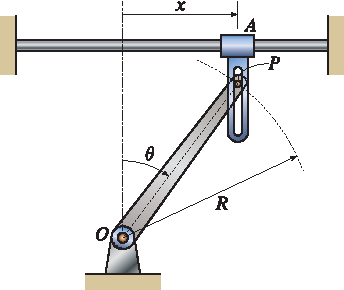
\includegraphics[width=3in]{Chapter-1/Figures/mechanism}
    \caption{We hold these truths to be self-evident, that all men are created equal,  that they are endowed by their Creator with certain unalienable Rights,  that among these are Life, Liberty and the pursuit of Happiness.}
    \label{Ch1-figure: mechanism}
\end{figure}
%%%
Check out Fig.~\ref{Ch1-figure: mechanism}!


\section{More Declaration}

We hold these truths to be self-evident, that all men are created equal,  that they are endowed by their Creator with certain unalienable Rights,  that among these are Life, Liberty and the pursuit of Happiness. That to secure these  rights, Governments are instituted among Men, deriving their just powers  from the consent of the governed, That whenever any Form of Government  becomes destructive of these ends, it is the Right of the People to alter  or to abolish it, and to institute new Government, laying its foundation on  such principles and organizing its powers in such form, as to them shall  seem most likely to effect their Safety and Happiness. Prudence, indeed, will dictate that Governments long established should not  be changed for light and transient causes; and accordingly all experience  hath shewn, that mankind are more disposed to suffer, while evils are  sufferable, than to right themselves by abolishing the forms to which they  are accustomed.
%%%
\begin{figure}[htb]
    \centering
%    \includegraphics{\FigPath{FigureFileName}}
    \caption{We hold these truths to be self-evident, that all men are created equal,  that they are endowed by their Creator with certain unalienable Rights,  that among these are Life, Liberty and the pursuit of Happiness.}
    \label{ChX-figure: FigureLabel3}
\end{figure}
%%%
But when a long train of abuses and usurpations, pursuing invariably the same  Object evinces a design to reduce them under absolute Despotism, it is their  right, it is their duty, to throw off such Government, and to provide new Guards for their future security. --Such has been the patient sufferance of these Colonies; and such is now the  necessity which constrains them to alter their former Systems of Government.  The history of the present King of Great Britain [George III] is a history  of repeated injuries and usurpations, all having in direct object the  establishment of an absolute Tyranny over these States. To prove this, let Facts be submitted to a candid world.